%
%
%
%
\section{Application: Automated Diagnosis and Active Learning} \label{sec:active-learning}
%

%
%
%
An important problem in AI is automated diagnosis. For example, suppose we have different hypotheses about the state of a patient, and can run medical tests to rule out inconsistent hypotheses. The goal is to adaptively choose tests to infer the state of the patient as quickly as possible.

A similar problem arises in active learning. Obtaining labeled data to train a classifier is typically expensive, as it often involves asking an expert. In active learning (\cf~\citet{cohn96active,mccallum98}), the key idea is that some labels are more informative than others: labeling a few unlabeled examples can imply the labels of many other unlabeled examples, and thus the cost of obtaining the labels from an expert can be avoided. As is standard, we assume that we are given a set of hypotheses $\hypotheses$,
and a set of unlabeled data points $\data$ where each $x \in \data$
is independently drawn from some
distribution $\distrib$.  Let $\labels$ be the set of possible labels.  
Classical learning theory yields \emph{probably approximately correct} (PAC) bounds, bounding the number $n$ of examples drawn i.i.d. from $\distrib$ needed to output a hypothesis $h$ that will have expected error at most $\eps$ with probability at least $1 - \delta$,
for some fixed $\eps, \delta > 0$.  That is, if $\target$ is the 
target hypothesis (with zero error), and 
$\error(h) := \probover{x \sim \distrib}{h(x) \neq \target(x)}$
is the error of $h$, 
 we require
$\prob{\error(h)  \le \eps } \ge 1 - \delta$.
The latter probability is taken with respect to $\distrib(\data)$;  the learned
hypothesis $h$ and thus $\error(h)$ depend on it.
A key challenge in active learning is to avoid bias: actively selected examples are no longer i.i.d., and thus sample complexity bounds for passive learning no longer apply.  If one is not careful, active learning may require more samples than passive learning to achieve the same generalization error.
One natural approach to active learning that is guaranteed to perform at least as well as passive learning is \emph{pool-based active learning} \citep{mccallum98}: The idea is to draw $n$ \emph{unlabeled} examples i.i.d. However, instead of obtaining all labels, labels are adaptively requested until the labels of all unlabeled examples are implied by the obtained labels. Now we have obtained $n$ labeled examples drawn i.i.d., and classical PAC bounds still apply. The key question is how to request the labels for the pool to infer the remaining labels as quickly as possible.




In the case of binary labels (or test outcomes) $L = \set{-1, 1}$, various authors have considered greedy
policies which generalize binary
search~\citep{garey74,loveland85,arkin93,kosaraju99,dasgupta04,guillory09,nowak09}.  
The simplest of these, called \emph{generalized binary search} (\gbs) or the
\emph{splitting algorithm}, works as follows.
Define the \emph{version
  space} \vs to be the set of hypotheses consistent with the observed
labels (here we assume that there is no label noise).
In the worst-case setting, \gbs selects a query $x \in
\data$ that minimizes $\left| \sum_{h \in \vs} h(x) \right|$. 
In the Bayesian setting we assume we are given a prior $\prior$ over
hypotheses; in this case \gbs selects a query $x \in
\data$ that minimizes $\left| \sum_{h \in \vs} \prior(h) \cdot h(x) \right|$.  Intuitively
these policies myopically attempt to shrink a measure of the version space (i.e., 
the cardinality or the probability mass) as quickly as
possible.
The former provides an $\cO(\log |\hypotheses|)$-approximation for the
worst-case number of queries~\citep{arkin93}, and the latter provides an 
 $\cO(\log \frac{1}{\min_{h} \prior(h)})$-approximation for the 
expected number of queries~\citep{kosaraju99,dasgupta04} and a natural
generalization of GBS obtains the same guarantees with a larger set of
labels~\citep{guillory09}. 
%
Kosaraju~\etal also prove that running GBS on a modified prior 
$\prior'(h) \propto \max\set{\prior(h), 1/|\hypotheses|^{2}\log
  |\hypotheses|}$ is sufficient to obtain an  $\cO(\log |\hypotheses|)$-approximation.


 \begin{figure} 
 \centering 
 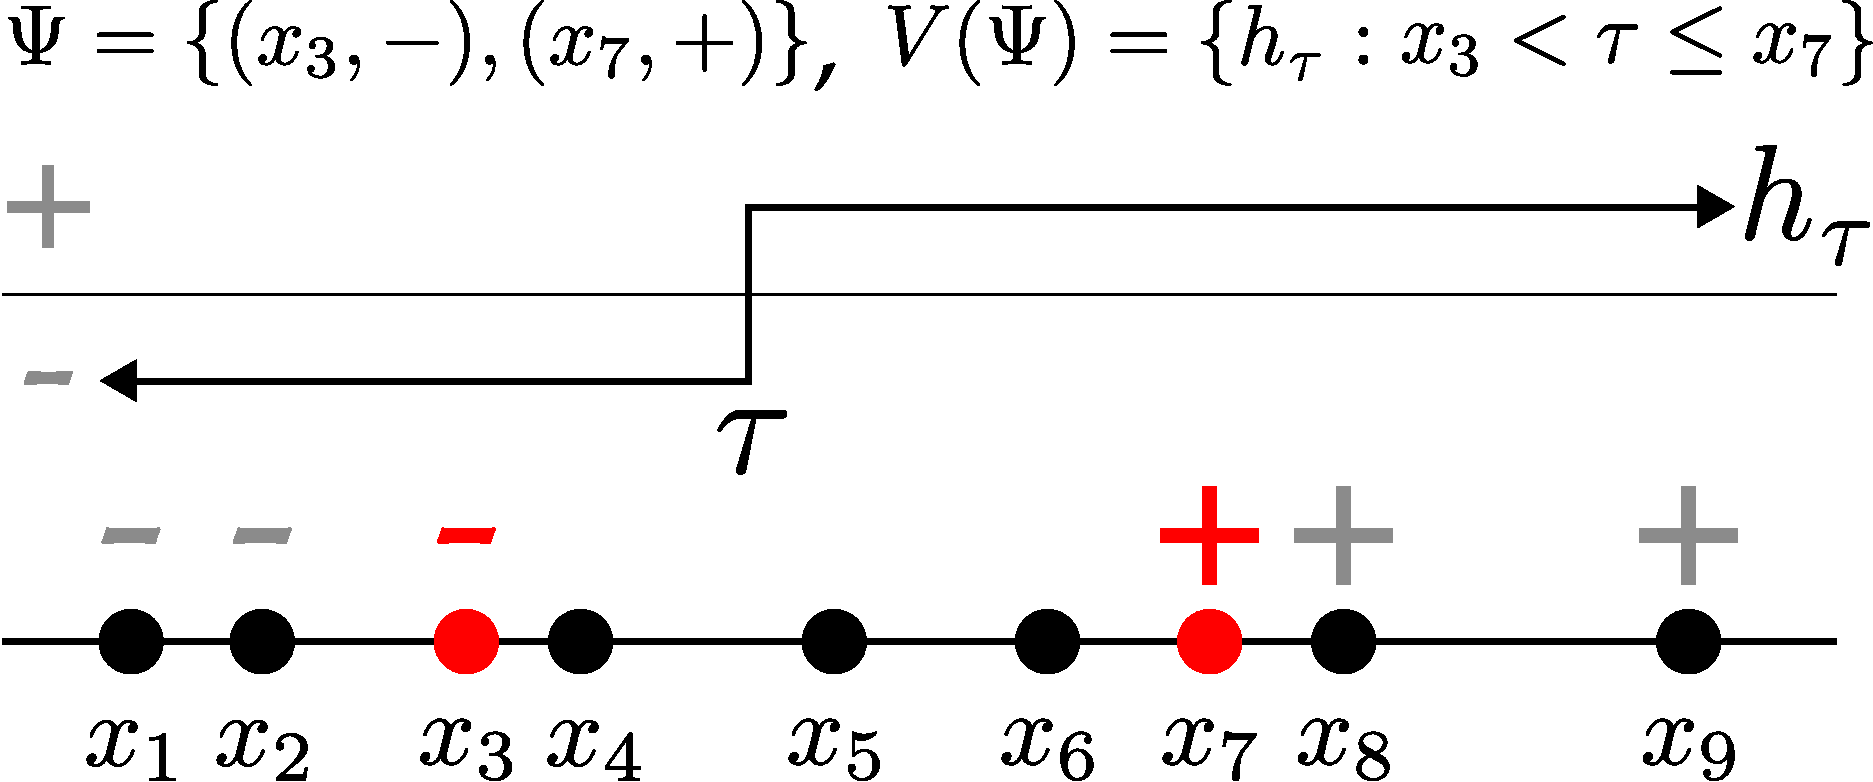
\includegraphics[width=0.6\textwidth]{figs/activeLearning}
 \caption{Illustration of the Active Learning problem, in the simple
   special case of one-dimensional data and 
binary threshold hypotheses $\hypotheses = \set{h_\tau : \tau \in
  \reals}$, where $h_\tau(x) = 1$ if $x \ge \tau$ and $0$ otherwise.
 \label{fig:activelearning}}
 \end{figure}


Viewed from this perspective of the previous sections, shrinking the
version space amounts to ``covering'' all false hypotheses with stochastic
sets (i.e., queries), where query $x$ covers all hypotheses that
disagree with the target hypothesis $\target$ at $x$.  That is, 
$x$ covers $\set{h : h(x) \neq \target(x)}$.  As
in~\secref{sec:viral-marketing}, these sets may be correlated in
complex ways determined by the set of possible hypotheses.
%
%
%
As we will show, the reduction in version space mass is \term
submodular, and this allows us to obtain 
%
a new analysis of GBS using \term submodularity, 
which is arguably more amenable to extensions
and generalizations than previous analyses.
Our new analysis further allows us to improve on the previous best bound on the approximation factor of GBS~\citep{dasgupta04} from 
$4 \,\ln \paren{\frac{1}{\min_{h}
  \prior(h)}}$ to $\ln \paren{\frac{1}{\min_{h}
  \prior(h)}} + 1$. 
We also show that when we apply GBS to a modified prior distribution,
the approximation factor is improved to $\cO(\ln |\hypotheses|)$. 
This result  matches a  lower bound of $\Omega(\ln |\hypotheses|)$ of
\citet{chakaravarthy07decision} 
up to constant factors. 


\begin{theorem} \label{thm:optimal-decision-trees}
%
  In the Bayesian setting in which there is a prior $\prior$ on a
  finite set of hypotheses $\hypotheses$, the generalized binary search algorithm
  makes $\OPT \cdot \paren{ \ln \paren{\frac{1}{\min_{h} \prior(h)}} + 1}$ queries in
  expectation to identify a hypothesis drawn from $\prior$, 
  where $\OPT$ is the minimum expected number of queries
  made by any policy.  
  If $\min_{h} \prior(h)$ is sufficiently small,
  running the algorithm on a modified prior 
$\prior'(h) \propto \max\set{\prior(h), 1/|\hypotheses|^{2}}$ improves the approximation factor to 
$\cO(\ln |\hypotheses|)$.
\end{theorem}

%
\looseness -1 

We devote the better part of the remainder of this section to the
proof of \thmref{thm:optimal-decision-trees}, which has several
components.
We first address the important special case of a uniform prior
over hypotheses, i.e., $\prior(h) = 1/|\hypotheses|$ for all $h \in
\hypotheses$, and then we reduce the case with a general prior to a
uniform prior.
We wish to appeal to Theorem~\ref{thm:min-set-cover-avg-generalized},
so we convert the problem into an Adaptive Stochastic Min Cost Cover problem.  

\subsection{The Reduction to Adaptive Stochastic Min Cost Cover}  
%
Define a realization $\rlz_h$ for each hypothesis $h \in \hypotheses$.
The ground set is $\groundset = \data$, and the
outcomes are binary; we define $\outcomes = \set{-1,1}$ instead of
using $\set{0,1}$ to be consistent with our earlier exposition.
For all $h\in \hypotheses$ we set $\rlz_h \equiv h$, meaning  
$\rlz_h(x) = h(x)$ for all $x \in \data$.
To define the objective function, we first need some notation.
Given observed labels $\prlz \subset \data \times \outcomes$, let
$\vs(\prlz)$ denote the version space, i.e., the set of hypotheses for
which $h(x) = \prlz(x)$ for all $x \in \dom(\prlz) $.
See \figref{fig:activelearning} for an illustration of an active
learning problem in the case of 
indicator hypotheses.
For a set of hypotheses $\vs$,  let $\prior(\vs) := \sum_{h \in \vs}
\prior(h)$ denote their total prior probability.
Finally, let $\prlz(S, h) = \set{(x, h(x)) \ : \ x \in S }$
be the function with domain $S$ that agrees with $h$ on $S$.
We define the objective function by 
\[
f(S, \rlz_h) \ :=  \ 1 - \prior(\vs(\prlz(S, h)  ) ) \ = \
\prior\!\paren{ \set{h' \ : \ \exists x \in S, h'(x) \neq h(x)}}
\]
and use $\rlzmass{\rlz_h} = \prior(h) = 1/|\hypotheses|$ for all $h$.
Let $\policy^*$ be an optimal policy for this 
Adaptive Stochastic Min Cost Cover instance.  Note that there is an exact correspondence between
policies for the original problem of finding the target hypothesis and
our problem of covering the true realization; $\target$ is identified as the target
hypothesis if and only if the version space is reduced to
$\set{\target}$ which occurs if and only if $\rlz_{\target}$ is covered.
Hence $\acst{\policy^*} = \OPT$.
Note that because we have assumed a uniform prior over hypotheses, we have 
$f(\data, \rlz_h) = 1 -  1/|\hypotheses|$ for all $h$.
Furthermore, the instances are \certifying.

\begin{lemma} \label{lem:active-learning-certifying}
The instances described above are \certifying for arbitrary priors $\prior$.   
\end{lemma}

\begin{proof}
Intuitively, theses instances are \certifying because to cover $\rlz_{\target}$ a
policy must identify $\rlz_{\target}$. More formally, these instances are \certifying because for any 
$\rlz_{h}$ and $\prlz$ such that $\rlz_{h} \sim \prlz$, we have that 
$f(\dom(\prlz), \rlz_{h}) = f(\data, \rlz_{h})$ implies 
$\vs(\prlz) = \set{h}$.   This in turn means that $\rlz_{h}$ is the \emph{only}
realization consistent with $\prlz$, which trivially implies that any
realization $\rlz' \sim \prlz$ also has $f(\dom(\prlz), \rlz') =
f(\data, \rlz')$; hence the instance is \certifying.
\end{proof}


\subsection{The Uniform Prior}  We next prove that the instances
generated are adaptive submodular and strongly adaptive
monotone under a uniform prior.


\begin{lemma} \label{lem:active-learning-adapt-submod-uniform}
In the instances described above, $f$ is strongly adaptive
monotone and \term submodular and with respect to a uniform prior $\prior$.
\end{lemma}

\begin{proof}
Demonstrating strong adaptive monotonicity under a uniform prior 
amounts to proving that adding labels
cannot grow the version space, which is clear in our model. 
That is, each query $x$ eliminates some subset of
hypotheses, and as more queries are performed, the subset of
hypotheses eliminated by $x$ cannot grow.  
%
Moving on to \term submodularity, consider the expected marginal contribution of $x$
under two partial realizations $\prlz, \prlz'$ where $\prlz$ is a
subrealization of $\prlz'$ (i.e., $\prlz \subset \prlz'$), and $x
\notin \dom(\prlz')$.
Let $\prlzxo$ be the partial
realization with domain $\dom(\prlz)  \cup \set{x}$ that agrees with
$\prlz$ on its domain, and maps $x$ to $\outcome$.
For each $\outcome \in \outcomes$, 
let 
$a_{\outcome} :=
\prior(\vs(\substitute{\prlz}{x}{\outcome}))$, $b_{\outcome} :=
\prior(\vs(\substitute{\prlz'}{x}{\outcome}))$.
Since a hypothesis eliminated from the version space cannot later
appear in the version space, we have 
$a_{\outcome} \ge b_{\outcome}$ for all $\outcome$.
Next, note the expected reduction in version space mass (and hence the expected
marginal contribution) due to selecting $x$ given partial realization
$\prlz$ is 
\begin{equation}
  \label{eq:active01}
  \diff{\prlz}{x} = \sum_{\outcome \in \outcomes} a_{\outcome} \cdot 
  \prob{\rvrlz(x) \neq \outcome \ \mid \ \rvrlz \sim \prlz} =
  \sum_{\outcome} a_{\outcome} \paren{\frac{ \sum_{\outcome' \neq
        \outcome} a_{\outcome'} }{  \sum_{\outcome'} a_{\outcome'}  }
  } = \frac{ \sum_{\outcome \neq \outcome'} a_{\outcome} a_{\outcome'} }{  \sum_{\outcome'} a_{\outcome'}}.
\end{equation}
The corresponding quantity for $\prlz'$ has $b_{\outcome}$ substituted
for $a_{\outcome}$ in~\eqnref{eq:active01}, for each $\outcome \in \outcomes$.
To prove \term submodularity
we must show 
$\diff{\prlz}{x} \ge \diff{\prlz'}{x}$ and to do so it suffices to show that $\partial
  \phi / \partial z_{\outcome} \ge 0$ for each $\outcome$ and 
$\vec{z} \in \set{\vec{c} \in [0,1]^{\outcomes} : \sum_{\outcome}
  c_{\outcome} > 0 }$, where 
$\phi(\vec{z}\,) :=  \paren{\sum_{\outcome \neq \outcome'} z_{\outcome}
  z_{\outcome'}} /  \paren{\sum_{\outcome'} z_{\outcome'}}$ has the
same functional form as the expression for $\diff{\prlz}{x}$ in~\eqnref{eq:active01}. 
 This is because $\partial\phi / \partial
z_{\outcome} \ge 0$ for each $\outcome$ implies that growing the version space
in any manner cannot decrease the expected marginal benefit of query $x$, and
hence shrinking it in any manner cannot increase the expected marginal benefit
of $x$. 
It is 
indeed the case that $\partial\phi / \partial
z_{\outcome} \ge 0$ for each $\outcome$.  More specifically, it holds that 
$$ 
\frac{\partial \phi}{\partial z_{a}} =  
\frac{\sum_{b \neq a} z_{b}^2
  +\sum_{(b, c) : b \neq c, b \neq a, c \neq a} z_{b}
  z_{c} }{ \paren{\sum_{b} z_{b}}^2  } \ge 0,$$
which can be derived through elementary calculus.
\end{proof}

Hence we can apply Theorem~\ref{thm:min-set-cover-avg-generalized} to
this \certifying instance with maximum reward threshold $Q =  1 -  1/|\hypotheses|$, and 
minimum gap $\eta = 1/|\hypotheses|$, to obtain an upper bound of 
$\OPT \paren{\ln \paren{|\hypotheses|-1} + 1}$ on the number of
queries made by the 
generalized binary search algorithm (which corresponds exactly to the greedy policy
for Adaptive Stochastic Min Cost Cover) 
under the assumption of a uniform
prior over $\hypotheses$.

\subsection{Arbitrary Priors} 
Now consider general priors over $\hypotheses$.  
We construct the 
Adaptive Stochastic Min Cost Cover 
instance as before, only we change the objective function to 
\begin{equation}
  \label{eq:active-learning-obj}
f(S, \rlz_h) \ :=  \ 1 - \prior(\vs(\prlz(S, h)  ) ) + \prior(h)\mbox{.}  
\end{equation}
First note that the instances remain \certifying.  The proof of \lemref{lem:active-learning-certifying}
goes through completely unchanged by the modification of $f$.  We proceed to
show adaptive submodularity and strong adaptive monotonicity.

\begin{lemma} \label{lem:active-learning-adapt-submod-arbitrary-priors}
The objective function $f$ as described in \eqnref{eq:active-learning-obj}
is strongly adaptive monotone and \term submodular and with respect to arbitrary priors $\prior$.
\end{lemma}

\begin{proof}
The modified objective is still \term submodular, because 
$(S, \rlz_h) \mapsto \prior(h)$ is clearly so, and because \term submodularity is defined
via linear inequalities it is preserved under taking nonnegative linear combinations. 
Note that $f(\data, \rlz_h) = 1$ for all $\rlz_h$.


Showing $f$ is strongly adaptive monotone requires slightly more
work than before.  
Fix $\prlz, x \notin \dom(\prlz)$, and
$\outcome \in \outcomes$.  We must show 
\begin{equation}
  \label{eq:active-learning2}
  \expctoverrlz{\rvrlz}{f(\dom(\prlz), \rvrlz) \ \mid \ \rvrlz \sim \prlz} \le 
\expctoverrlz{\rvrlz}{f(\dom(\prlz) \cup \set{x}, \rvrlz) \ \mid \ \rvrlz \sim
  \prlz, \rvrlz(x) = \outcome}.  
\end{equation}
Plugging in
the definition of $f$, the
inequality we wish to prove may be simplified to 
\begin{equation}
  \label{eq:active1}
  \expctoverrlz{\rvrlz}{\prior(\rvrlz) \ \mid \ \rvrlz \sim \prlz} -
\expctoverrlz{\rvrlz}{\prior(\rvrlz) \ \mid \ \rvrlz \sim \prlzxo} \ 
\le \ \prior(\vs(\prlz)) - \prior(\vs(\prlzxo))\mbox{.}
\end{equation}
where $\rvrlz$ is the random realization of the hypothesis, and 
$\prior(\rlz_h) = \prior(h)$ for all $h$. 
Let $\vselim := \vs(\prlz) - \vs(\prlzxo)$ be the set of hypotheses
eliminated from the version space by the observation $h(x) = \outcome$.
Rewriting \eqnref{eq:active1}, we get 
\begin{equation}
  \label{eq:active2}
\sum_{h \in \vs(\prlz)} \frac{\prior(h)^2}{\prior(\vs(\prlz))} \ 
- \sum_{h \in \vs(\prlzxo)}
  \frac{\prior(h)^2}{\prior(\vs(\prlzxo))} \ \le \ \prior(\vselim)
\mbox{.}
\end{equation}
Let $\operatorname{LHS}_{\ref{eq:active2}}$ denote the left hand side
of~\eqnref{eq:active2}.  We prove~\eqnref{eq:active2}  as follows.
\[
\begin{array}{lclr}
\operatorname{LHS}_{\ref{eq:active2}} 
& \le &  \sum_{h \in
    \vselim} \prior(h)^2 / \prior(\vs(\prlz)) &
  [\text{since }\prior(\vs(\prlzxo)) \le \prior(\vs(\prlz)) ]\vspace{2mm}\\
 & \le & \sum_{h \in
    \vselim} \prior(h) \cdot
    \prior(\vs(\prlz)) / \prior(\vs(\prlz)) & \hspace{0mm} [\text{since } h \in
  \vs(\prlz) \implies \prior(h)
  \le \prior(\vs(\prlz))  ]\vspace{2mm}\\
 & = &  \prior(\vselim) & \\
\end{array}
\]

\noindent We conclude that $f$ is \term submodular and strongly
adaptive monotone.
\end{proof}


Hence we can apply Theorem~\ref{thm:min-set-cover-avg-generalized} to
this \certifying instance 
with maximum reward threshold $Q =  1$, and 
minimum gap $\eta = 1/\min_{h} \prior(h)$.   As a result we obtain an upper bound of 
$\OPT \paren{\ln \paren{1/\min_{h} \prior(h)} + 1}$ on the number of
queries made by 
generalized binary search for arbitrary priors, completing the proof
of \thmref{thm:optimal-decision-trees}.

\subsection{Improving the Approximation Factor for Highly Nonuniform Priors}
To improve this to an $\cO(\log |\hypotheses|)$-approximation in the
event that $\min_{h} \prior(h)$ is extremely small 
using the
observation of~\citet{kosaraju99}, call a policy $\policy$
\emph{progressive} if it eliminates at least one hypothesis from its
version space in each query.  Let 
$\prior'(h) =  \max\set{\prior(h),
  1/|\hypotheses|^{2}}/Z$ 
be the modified prior, where $Z := \sum_{h'}  \max\set{\prior(h'),
  1/|\hypotheses|^{2}}$ is the normalizing constant.
Let $\c(\policy, h)$ be the cost (i.e., \# of queries) of $\policy$ under target $h$.  Then 
$\acst{\policy, p} := \sum_{h} \c(\policy,h) p(h)$ is the expected cost of $\policy$
under prior $p$.
We will show that $\acst{\policy, \prior'}$ is a good approximation to
$\acst{\policy, \prior}$.
%
Call $h$ \emph{rare} if $\prior(h) < 1/|\hypotheses|^{2}$, and
\emph{common} otherwise.
First, note that $\sum_{h'}  \max\set{\prior(h'), 1/|\hypotheses|^{2}}
\le 1 + 1/|\hypotheses|$, and so 
$\prior'(h) \ge \frac{|\hypotheses|}{|\hypotheses| + 1} \prior(h)$,
for all $h$.   Hence for all $\policy$, we have 
$\acst{\policy, \prior'} \ge \frac{|\hypotheses|}{|\hypotheses| + 1} \acst{\policy, \prior}$.
%
Next, we show $\acst{\policy, \prior'} \le \acst{\policy, \prior} + 1$.
Consider the quantity $\acst{\policy, \prior'} - \acst{\policy, \prior} =  \sum_{h}
\c(\policy,h) \paren{\prior'(h) - \prior(h)}$.
The positive contributions must come from rare hypotheses.
However, the total probability mass of these under $\prior'$ is at
most $1/|\hypotheses|$, and since $\policy$ is progressive 
$\c(\policy,h) \le |\hypotheses|$ for all $h$, hence the difference in costs is at most one.
Let $\alpha := \ln \paren{\frac{1}{\min_{h} \prior'(h)}} + 1 \le
\ln \paren{|\hypotheses|^2 + |\hypotheses|} + 1$ be the approximation
factor for generalized binary search when run on $\prior'$.  
Let $\policy$ be the policy of generalized binary search, and
let $\policy^*$ be an optimal policy under prior $\prior$.
Then 
\[
\acst{\policy, \prior} \le \frac{|\hypotheses|+1}{|\hypotheses|} \,\acst{\policy,
  \prior'} 
\le \frac{|\hypotheses|+1}{|\hypotheses|} \, \alpha \, \acst{\policy^*,
  \prior'} \le  \frac{|\hypotheses|+1}{|\hypotheses|} \, \alpha \, \paren{\acst{\policy^*, \prior} + 1}.
\]
With some further algebra, we can derive $\acst{\policy, \prior}
\le \paren{\acst{\policy^*, \prior} + 1} \paren{\ln \paren{ 2e |\hypotheses|^2}}$.
Thus for a general prior a simple modification of GBS 
yields an $\cO(\log |\hypotheses|)$-approximation.



\subsection{Extensions to Arbitrary
  Costs, Multiple Classes, and Approximate Greedy Policies}  
This result easily generalizes to handle 
the setting of multiple classes / test outcomes  (i.e., $|\outcomes| \ge 2$), and
$\alpha$-approximate greedy policies, where we lose a factor of
$\alpha$ in the approximation factor.  
As we describe
in \appendixA,
we can 
generalize \term submodularity to incorporate costs on items,
which allows us to extend this result to handle query costs as well.   
We can therefore
recover these extensions 
of~\citet{guillory09}, while improving the approximation factor
for GBS with item costs 
to $\ln \paren{\frac{1}{\min_{h}  \prior(h)}} + 1$.  
\citeauthor{guillory09} 
also showed how to extend the
technique of~\citet{kosaraju99} to obtain an $\cO\paren{\log
\paren{|\hypotheses|\frac{\max_{x} c(x)}{\min_{x}
    c(x)}}}$-approximation with costs using a greedy policy, which
may be combined with our tighter analysis 
as well to give a similar result with an improved leading constant.
%
Recently, \citet{gupta10approximation} showed how to simultaneously remove the
dependence on both costs and probabilities from the approximation ratio.
Specifically, within the context of studying an adaptive travelling
salesman problem 
they investigated the \emph{Optimal Decision Tree} problem, which is
equivalent to the active learning problem we consider here.  Using a clever, more
complex algorithm than adaptive greedy, 
they achieve an $\cO\paren{\log |\hypotheses|}$-approximation
in the case of non-uniform  costs and general priors.  

\subsection{Extensions to Active Learning with Noisy Observations}  
\thmref{thm:optimal-decision-trees} and the extensions mentioned so far
are in the noise free case, i.e., the result of query $x$ and observes
$\target(x)$, where $\target$ is the target hypothesis.
Many practical problems may have \emph{noisy} observations.
\citet{nowak09} considered the case in which the outcomes are binary,
i.e., $\outcomes = \set{-1,1}$, the same query may be asked multiple
times, and for each instance of each query the noise is independent.
In this case he gives performance guarantees for generalized binary
search.  While this setting may be appropriate if the noise is due to
measurement error, in some applications the noise is
\emph{persistent}, i.e., if query $x$ is asked several times, the observation
is always the same.  Recently, \citet{golovin10nips}
and~\citet{bellala10modified} have used the adaptive submodularity framework to obtain 
the first algorithms with provable (logarithmic) approximation guarantees for 
active learning with persistent noise.


%
%
%
%
%
